\section{Ejercicio 03}

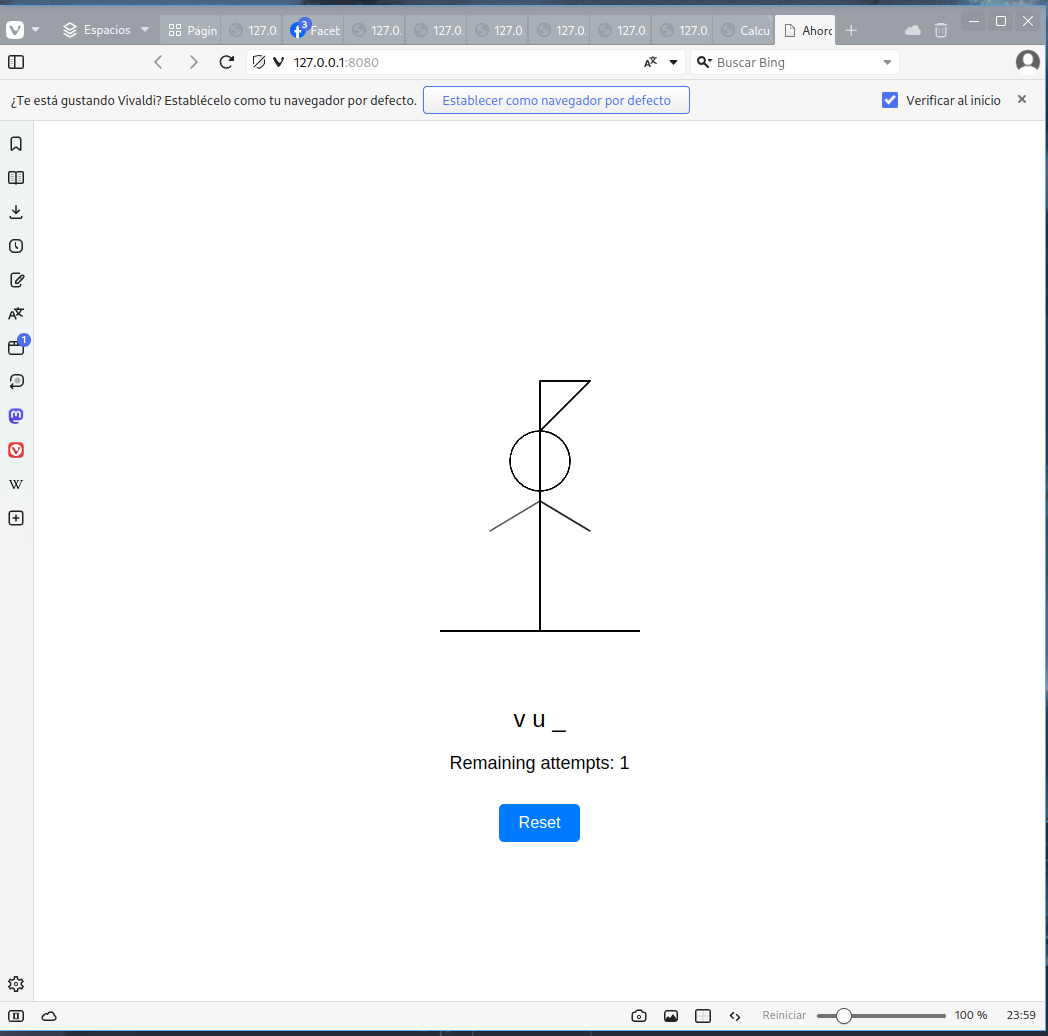
\includegraphics[width=1\textwidth]{./img/ejercicio03.png}

Aqui veremos la lógica principal del juego. Veamos el código paso a paso:

\begin{lstlisting}[language=JavaScript]
const canvas = document.getElementById('hangmanCanvas');
const ctx = canvas.getContext('2d');
\end{lstlisting}

Se obtienen referencias al elemento del canvas (canvas) y su contexto de dibujo 2D (ctx).

\begin{lstlisting}[language=JavaScript]
var wordContainer = document.getElementById('word-container');
var guessesContainer = document.getElementById('guesses-container');
var resetButton = document.getElementById('reset-button');
\end{lstlisting}

Se obtienen referencias a los elementos del DOM que mostrarán la palabra a adivinar (wordContainer), las letras adivinadas (guessesContainer) y el botón de reinicio (resetButton).

\begin{lstlisting}[language=JavaScript]
const words = ['javascript', 'html', 'css', 'python', 'react', 'angular', 'vue'];
let selectedWord = words[Math.floor(Math.random() * words.length)];
let guessedLetters = [];
let remainingAttempts = 6;
\end{lstlisting}

Se define un array de palabras (words) para elegir una aleatoriamente. Se selecciona una palabra aleatoria del array (selectedWord). Se inicializa un array vacío para almacenar las letras adivinadas (guessedLetters). Se define la cantidad inicial de intentos restantes (remainingAttempts).

\textbf{Funciones del juego:}

\textbf{- \texttt{drawHangman()}:} Esta función dibuja el ahorcado en el canvas en base a la cantidad de intentos restantes.

\textbf{- \texttt{displayWord()}:} Esta función muestra la palabra a adivinar en el elemento wordContainer. Si una letra ya ha sido adivinada, se muestra la letra, sino se muestra un guión bajo.

\textbf{- \texttt{displayGuesses()}:} Esta función muestra el número de intentos restantes en el elemento guessesContainer.

\textbf{- \texttt{checkWin()}:} Esta función verifica si el jugador ha ganado. Recorre la palabra seleccionada y verifica si todas las letras están incluidas en el array de letras adivinadas.

\textbf{- \texttt{checkLose()}:} Esta función verifica si el jugador ha perdido. Simplemente compara si la cantidad de intentos restantes es igual a cero.

\textbf{- \texttt{guessLetter(letter)}:} Esta función maneja las pulsaciones de teclas del usuario. Recibe una letra como parámetro y verifica si:
  - La letra no ha sido adivinada previamente.
  - La letra está incluida en la palabra seleccionada.
  - Si la letra no está en la palabra, se resta un intento. Se actualiza el dibujo del ahorcado, se muestra la palabra actualizada y los intentos restantes.
  - Si se adivina la palabra completa, se muestra un mensaje de victoria y se reinicia el juego.
  - Si se pierden todos los intentos, se muestra la palabra y se reinicia el juego.

\textbf{- \texttt{resetGame()}:} Esta función reinicia el juego seleccionando una nueva palabra aleatoria, vaciando las letras adivinadas, reiniciando los intentos y actualizando la pantalla.

\textbf{Eventos:}

\begin{lstlisting}[language=JavaScript]
document.addEventListener('keydown', event => {...})
\end{lstlisting}

Escucha eventos de presión de teclas. Si la tecla presionada es una letra del alfabeto, se llama a la función guessLetter con la letra presionada en minúsculas.

\begin{lstlisting}[language=JavaScript]
resetButton.addEventListener('click', resetGame)
\end{lstlisting}

Escucha el click en el botón de reinicio y llama a la función resetGame.

\section*{components.js}

Este archivo se encarga de crear dinámicamente los elementos HTML necesarios para el juego y organizarlos en la página.

\begin{lstlisting}[language=JavaScript]
// Crear el contenedor del juego
var gameContainer = document.createElement("div");
gameContainer.id = "game-container";

// ... (se crean el canvas, los contenedores para la palabra, letras adivinadas y botón de reinicio)

// Agregar el contenedor del juego al body
document.body.appendChild(gameContainer);
\end{lstlisting}

Se crea un elemento div con el identificador game-container que servirá como contenedor principal del juego. Se crean individualmente los elementos para el canvas (hangmanCanvas), los contenedores de texto (wordContainer y guessesContainer) y el botón de reinicio (resetButton). Se añaden todos los elementos creados como hijos del contenedor principal (gameContainer). Finalmente, se añade el contenedor principal (gameContainer) como hijo del elemento body del documento HTML.

\section*{styles.js}

Este archivo define los estilos CSS para los elementos del juego.

\begin{lstlisting}[language=JavaScript]
// Establecer estilos para el body
document.body.style.fontFamily = 'Arial, sans-serif';
document.body.style.display = 'flex';
document.body.style.justifyContent = 'center';
document.body.style.alignItems = 'center';
document.body.style.height = '100vh';
document.body.style.margin = '0';

// Establecer estilos para el contenedor del juego
var gameContainer = document.getElementById('game-container');
gameContainer.style.textAlign = 'center';

// Establecer estilos para el contenedor de la palabra
var wordContainer = document.getElementById('word-container');
wordContainer.style.margin = '20px 0';
wordContainer.style.fontSize = '24px';

// Establecer estilos para el contenedor de las letras adivinadas
var guessesContainer = document.getElementById('guesses-container');
guessesContainer.style.margin = '10px 0';
guessesContainer.style.fontSize = '18px';

// Establecer estilos para el botón de reset
var resetButton = document.getElementById('reset-button');
resetButton.style.marginTop = '20px';
resetButton.style.padding = '10px 20px';
resetButton.style.fontSize = '16px';
resetButton.style.backgroundColor = '#007bff';
resetButton.style.color = 'white';
resetButton.style.border = 'none';
resetButton.style.borderRadius = '5px';
resetButton.style.cursor = 'pointer';

// Establecer estilos para el hover del botón de reset
resetButton.addEventListener('mouseover', () => {
  resetButton.style.backgroundColor = '#0056b3';
});

resetButton.addEventListener('mouseout', () => {
  resetButton.style.backgroundColor = '#007bff';
\end{lstlisting}
Se establecen estilos globales para el elemento body del documento HTML, centrando el contenido y definiendo una altura del 100\% del viewport. Se definen estilos para el contenedor principal del juego (gameContainer), centrando el texto dentro de él. Se definen estilos para los contenedores de la palabra (wordContainer) y las letras adivinadas (guessesContainer), ajustando márgenes y tamaño de letra. Se definen estilos para el botón de reinicio (resetButton).
